\documentclass[10pt,a4paper]{article}
\usepackage[utf8]{inputenc}
\usepackage[spanish]{babel}
\usepackage{amsmath}
\usepackage{amsfonts}
\usepackage{amssymb}
\usepackage{graphics}
\usepackage{graphicx}
\usepackage{xcolor}
\usepackage{listings}
\usepackage{csvsimple}
\usepackage{caption}
\usepackage{subcaption}
\usepackage[left=2cm,right=2cm,top=2cm,bottom=2cm]{geometry}

\renewcommand*\contentsname{Índice} %Nombre del indice

\begin{document}
\lstset{
	basicstyle=\footnotesize,
	extendedchars=true,
	literate={á}{{\'a}}1 {ã}{{\~a}}1 {é}{{\'e}}1 {ú}{{\'u}}1 {ó}{{\'o}}1,
	backgroundcolor=\color{black!5}
	}
	
\begin{titlepage}
	\centering
	{
\includegraphics[scale=0.5]{Logo_UGR.png}\par}
	\vspace{1cm}
	{\bfseries\Large Escuela T\'ecnica Superior de Ingeniería Informática y Telecomunicaciones \par}
	\vspace{2.5cm}
	{\scshape\Huge Pr\'actica 3: Algoritmos Greedy \par}
	\vspace{3cm}
	{\itshape\Large Doble Grado Ingeniería Informática y Matemáticas}
	\vfill
	{\Large Autores: \par}
	{\Large Jose Alberto Hoces Castro\par}
	{\Large Javier Gómez López \par}
	{\Large Moya Mart\'in Castaño \par}
	\vfill
	{\Large Mayo 2022 \par}
\end{titlepage}

\thispagestyle{empty}
\null
\vfill

%%Información sobre la licencia
\parbox[t]{\textwidth}{
  
\includegraphics[scale=0.05]{by-nc-sa.png}\\[4pt]
  \raggedright % Texto alineado a la izquierda
  \sffamily\large
  {\Large Este trabajo se distribuye bajo una licencia CC BY-NC-SA 4.0.}\\[4pt]
  Eres libre de distribuir y adaptar el material siempre que reconozcas a los\\
  autores originales del documento, no lo utilices para fines comerciales\\
  y lo distribuyas bajo la misma licencia.\\[4pt]
  \texttt{creativecommons.org/licenses/by-nc-sa/4.0/}
}

\newpage

\tableofcontents

\newpage

\section{Introducción}

El objetivo de esta práctica es aprender a implementar y utilizar algoritmos \textit{``greedy''} o voraces para resolver problemas de manera rápida aunque no por ello menos óptima. Para ello, se plantean los siguientes dos problemas:

\begin{itemize}
	\item \textbf{Ejercicio 1} (Contenedores): Se quiere rellenar un buque mercante con una cierta capacidad de peso con contenedores, cada uno de los cuales tiene su propio peso.
	\item \textbf{Ejercicio 2} (TSP): El problema del viajero. Se quiere recorrer una serie de ciudades, pasando por ellas solo una vez y volviendo al punto de partida. Se quiere encontrar la ruta más óptima.
\end{itemize}

\section{Desarrollo}

Para el primer ejercicio, nos centraremos en identificar el problema de los contenedores como un problema Greedy identificando sus características. También, justificaremos los optimalidad o la no optimalidad de los algoritmos Greedy desarrollados.
\\
\\
Para el análisis de los algoritmos del viajante de comercio que desarrollaremos, hemos realizado los siguientes pasos:

\begin{enumerate}
	\item Un \textbf{análisis teórico} donde se comentará el código desarrollado para la resolución de los problemas propuestos.
	
	\item Un \textbf{análisis empírico} donde hemos ejecutado los algoritmos en nuestros ordenadores bajo las mismas normas y condiciones. Hemos compilado usando la optimización \texttt{-Og}. Además, hemos usado como \textit{datasets} de pruebas los datos proporcionados por la profesora en el caso del TSP, y valores aleatorios de los pesos de los contenedores para el primer problema. Por otro lado, para automatizar el proceso, hemos creado unos \textit{scripts} de generació  de datos de prueba y de ejecución de nuestros programas. Hemos ejecutado cada algoritmo 15 veces en cada uno de los tamaños probados, y hemos hecho la media de ellos para reducir perturbaciones que puedan alterar el resultado.
	
	\item Un \textbf{análisis híbrido} donde hemos tomado los datos de cada uno de los alumnos del grupo y hemos hallado la \(K\) (constante oculta). Para ello hemos usado gnuplot.
\end{enumerate}

\subsection{Ejercicio 1. Contenedores}

El enunciado del problema es el siguiente: \textit{Se tiene un buque mercante cuya capacidad de carga es de } K \textit{toneladas y un conjunto de contenedores \(c_1, \dotsc, c_n\) cuyos pesos respectivos son \(p_1, \dotsc, p_n\) (expresados también en toneladas). Teniendo en cuenta que la capacidad del buque es menor que la suma total de los pesos de los contenedores: }

\begin{itemize}
	\item \textit{Diseñe un algoritmo que maximice el número de contenedores cargados, y demuestre su optimalidad.}
	\item \textit{Diseñe un algoritmo que intente maximizar el número de toneladas cargadas.}
\end{itemize}

\subsubsection{Primer ejercicio}
	Nuestro objetivo es que podamos cargar el máximo número de contenedores en un buque mercante de K toneladas. Para ello, el algoritmo que nosotros proponemos es tomar los contenedores, ordenarlos de menor a mayor peso, y comenzar añadiendo los de menor peso. De esta forma, podemos cargar más contenedores, ya que si empezásemos por los de pesos intermedios o mayores, acabaríamos cargando menos. 
	\\
	\\
	Veamos las 6 características de nuestro problema Greedy:
	\begin{itemize}
		\item \textbf{Un conjunto de candidatos}: En este caso, los contenedores a cargar.
		\item \textbf{Una lista de candidatos ya usados}: Los contenedores que ya han sido cargados.
		\item \textbf{Un criterio que dice cuándo un conjunto de candidatos forma una solución}: El criterio es que la suma de los pesos de un conjunto de contenedores no sea superior a las K toneladas del buque.
		\item \textbf{Un criterio que dice cuándo un conjunto de candidatos es factible (podrá llegar a ser una solución)}: el conjunto de contenedores que se evalúe no debe superar en peso las K toneladas del buque.
		\item \textbf{Una función de selección que indica en cualquier instante cuál es el candidato más prometedor de los no usados todavía}: El contenedor de menor peso de los que aún no están cargados, de ahí que los ordenemos de menor a mayor peso.
		\item \textbf{La función objetivo que intentamos optimizar}: El número de contenedores a cargar, es lo que queremos maximizar.
	\end{itemize}

	A continuación pasamos a mostrar el código de nuestro algoritmo. Para representar el conjunto de contenedores, hemos considerado un vector de enteros, siendo cada entero el peso de cada contenedor. Para asegurarnos de que la suma de los pesos de todos los contenedores supera a las K toneladas del buque, el vector es de dimensión K con enteros aleatorios desde 0 hasta K (en nuestro código lo representamos por el parámetro n, introducido por el usuario). Nuestra función devuelve el número de contenedores que se han podido cargar:
	
	\lstinputlisting[language=C++]{./Codes/contenedores1.cpp}
	
	\begin{itemize}
		\item \textbf{Estudio de la optimalidad}
		\\
		\\
		Vamos a probar la optimalidad de nuestro algoritmo mediante una demostración matemática. Sea $T = \lbrace c_{1},...,c_{n} \rbrace$ y llamemos $S = \lbrace c_{1},...,c_{m} \rbrace$ a la solución de nuestro algoritmo Greedy. Vamos a fijar notación para lo que sigue:
		
		\begin{itemize}
			\item $|S| \rightarrow$ Cardinal del conjunto de contenedores S
			\item $c_{i} \rightarrow$ Contenedor i
			\item $p_{i} \rightarrow$ Peso del contenedor i
		\end{itemize}
	
	Consideramos que $|S| = m$. Por cómo hemos diseñado el algoritmo, sabemos que los pesos de los contenedores de la solución cumplen que:
	
	\[
	\sum_{c_{i} \in S}p_{i} = \sum_{i = 1}^{m}p_{i} \leq  K \hspace{0.2cm} \text{y} \hspace{0.2cm} \sum_{i = 1}^{m+1}p_{i} > K
	\]
	
	También, dado un conjunto Q cualquiera no vacío que no está contenido en S, deducimos de lo anterior que:
	
	\[
	\sum_{c_{i} \in S}p_{i} + \sum_{c_{i} \in Q}p_{i} > K
	\]
	
	Para ver que nuestra solución es óptima, vamos a ver que dado cualquier subconjunto U de T con un cardinal mayor que S, es decir, con más contenedores que S ($|U| = m' > m = |S|$), nunca podrá ser solución del problema. Para ver que no es solución del problema, hay que probar que $\sum_{c_{i} \in U}p_{i} > K$.
	
	Comenzaremos descomponiendo el conjunto de contenedores U de una forma que nos interesa. Sabemos que $U = (S \cap U) \cup (U\setminus S)$. Por ello, podemos escribir la siguiente igualdad:
	
	\[
	\sum_{c_{i} \in U}p_{i} = \sum_{c_{i} \in S \cap U}p_{i} + \sum_{c_{i} \in U \setminus S}p_{i} 
	\]
	
	Debido a esto, $|U| = m' = |S \cap U| + |U\setminus S|$. También se tiene que $(S \cap U) \cup (S\setminus U)$, luego $|S| = m = |S \cap U| + |S\setminus U|$. Teniendo en cuenta las dos igualdades en términos de cardinales que acabamos de ver, se tiene que $|U \setminus S| = m' - |S \cap U| > m - |S \cap U| = |S \setminus U|$. Esto nos demuestra que en $|U \setminus S|$ hay más elementos que en $|S \setminus U|$.
	
	A continuación, consideramos un subconjunto R de $U \setminus S$ cuyo cardinal coincida con el de $S \setminus U$ (esto lo podemos hacer porque hemos demostrado antes que $|U \setminus S| > |S \setminus U|$), de forma que $U \setminus S \setminus R \neq \emptyset$. Esto nos permite seguir desarrollando la igualdad anterior:
	
	\[
	\sum_{c_{i} \in S \cap U}p_{i} + \sum_{c_{i} \in U \setminus S}p_{i} = \sum_{c_{i} \in S \cap U}p_{i} + \sum_{c_{i} \in R}p_{i} + \sum_{c_{i} \in U \setminus S \setminus R}p_{i}
	\]
	
	Ahora, hemos de tener en cuenta que todos los contenedores de $U \setminus S$ son de mayor peso que los de $S \setminus U$, y como R es subconjunto de $U \setminus S$, se cumple concretamente para los contenedores de R. Esto nos permite afirmar que la siguiente desigualdad es cierta (recordar que esto también se debe a que R y $S \setminus U$ tienen el mismo cardinal):
	
	\[
	\sum_{c_{i} \in S \cap U}p_{i} + \sum_{c_{i} \in R}p_{i} + \sum_{c_{i} \in U \setminus S \setminus R}p_{i} \geq \sum_{c_{i} \in S \cap U}p_{i} + \sum_{c_{i} \in S \setminus U}p_{i} + \sum_{c_{i} \in U \setminus S \setminus R}p_{i}
	\]
	
	Y el miembro de la derecha lo podemos reescribir como:
	
	\[
	\sum_{c_{i} \in S \cap U}p_{i} + \sum_{c_{i} \in S \setminus U}p_{i} + \sum_{c_{i} \in U \setminus S \setminus R}p_{i} = \sum_{c_{i} \in S}p_{i} + \sum_{c_{i} \in U \setminus S \setminus R}p_{i}
	\]
	
	Y por ser S la solución de nuestro algoritmo Greedy, sabemos que $\sum_{c_{i} \in S}p_{i} + \sum_{c_{i} \in U \setminus S \setminus R}p_{i} > K$, y si seguimos la secuencia de igualdades y la desigualdad final que hemos ido exponiendo, uniendo los extremos, llegamos a que $\sum_{c_{i} \in U}p_{i} > K$, que era lo que queríamos demostrar. Por tanto, S es la solución óptima del problema.
\end{itemize}
	
\subsubsection{Segundo ejercicio}

	En este segundo ejercicio, lo que queremos es maximizar las toneladas cargadas en el buque sin sobrepasar su capacidad total. Para ello, seguimos el pensamiento inverso al planteado en el anterior ejercicio. Como lo que nos interesa es cargar el máximo de toneladas posibles, empezaremos cargando aquellos contenedores cuyo peso sea el más grande. Para ello, los ordenamos de mayor a menor peso, justo al contrario que antes. Identificamos las 6 características de un problema Greedy:
	
	\begin{itemize}
		\item \textbf{Un conjunto de candidatos}: En este caso, los contenedores a cargar.
		\item \textbf{Una lista de candidatos ya usados}: Los contenedores que ya han sido cargados.
		\item \textbf{Un criterio que dice cuándo un conjunto de candidatos forma una solución}: El criterio es que la suma de los pesos de un conjunto de contenedores no sea superior a las K toneladas del buque.
		\item \textbf{Un criterio que dice cuándo un conjunto de candidatos es factible (podrá llegar a ser una solución)}: el conjunto de contenedores que se evalúe no debe superar en peso las K toneladas del buque.
		\item \textbf{Una función de selección que indica en cualquier instante cuál es el candidato más prometedor de los no usados todavía}: El contenedor de mayor peso de los que aún no están cargados, de ahí que los ordenemos de mayor a menor peso.
		\item \textbf{La función objetivo que intentamos optimizar}: El número de toneladas a cargar, es lo que queremos maximizar.
	\end{itemize}

	En el código del algoritmo, al igual que antes, simulamos los contenedores con sus respectivos pesos con un vector de enteros, el cual ordenamos de mayor a menor usando el sort de la STL. Se van sumando los pesos hasta que se sobrepase el tope de toneladas del buque. Nuestra función devuelve el número de toneladas que se han podido cargar en total:
	
	\lstinputlisting[language=C++]{./Codes/contenedores2.cpp}
	
	\begin{itemize}
		\item \textbf{Estudio de la optimalidad}
		\\
		\\
		Sin embargo, en este caso nuestro algoritmo no nos da la solución óptima. Veámoslo con un contraejemplo. Con n = 10, imaginemos que tenemos el vector [5, 4, 6, 1, 1, 2, 7, 9, 8, 3].
		Nuestro algoritmo lo ordenaría de mayor a menor, obteniendo el vector [9, 8, 7, 6, 5, 4, 3, 2, 1, 1]. Tras esto, se incluiría el contenedor de peso 9, pero el siguiente ya no sería posible cargarlo ya que 9 + 8 = 17 $>$ 10. La solución óptima en este caso sería tomar un contenedor de peso 1, otro de 2, otro de 3 y otro de 4, aprovechando así las 10 toneladas en su totalidad.
	\end{itemize}
	
\subsection{Ejercicio 2. El problema del viajante de comercio}

El enunciado del problema es el siguiente: \textit{dado un conjunto de ciudades y una matriz con las distancias entre todas ellas, un viajante debe recorrer todas las ciudades exactamente una vez, regresando al punto de partida, de forma tal que la distancia recorrida sea mínima.}

Además, se nos pide enfocarlo usando dos heurísticas distintas:
\begin{itemize}
	\item \textbf{Vecino más cercano}: dada una ciudad inicial \(v_0\), se agrega como ciudad siguiente aquella \(v_i\) (no incluida en el circuito) que se encuentre más cercana a \(v_0\). El procedimiento se repite hasta que todas las ciudades se hayan visitado.
	\item \textbf{Inserción}: la idea es comenzar con un recorrido parcial, que incluya algunas de las ciudades, y luego extender este recorrido insertando las ciudades restantes mediante algún criterio de tipo greedy.
\end{itemize}

Además, se debe proponer por parte del equipo otra heurística propia para resolver el problema.

\subsubsection*{Elementos comunes}
A lo largo de la solución del problema usaremos la siguiente notación para todas las heurísticas a desarrollar:
\begin{itemize}
	\item \(n\) es el \textbf{número de ciudades}.
	\item \(D\) es la \textbf{matriz de distancias}.
	\item \(r\) es el \textbf{vector de recorrido}, que contiene unra ruta que pasa por todas las ciudades, es decir, \(n\) elementos no repetidos.
	\item \(W_r\) es el \textbf{coste} de un recorrido, es decir, la distancia de un recorrido \(r\).
\end{itemize}

Adicionalmente, se han implementado una serie de funciones comunes a todas las heurísticas trabajadas en esta práctica:

\lstinputlisting[language=Python]{./Codes/common_functions.py}

Hemos definido una ``estructura'' \texttt{Point} para representar los puntos, una función \texttt{parse\_input} para parsear el input según el formato dado en los archivos de clase, \texttt{distance} que mide la distancia entre dos puntos, \texttt{gen\_distance\_matrix} que genera la matriz de distancias dada una lista de puntos y \texttt{get\_road\_distance} que da la longitud de un vector de recorrido.

Cabe destacar que los datos que se van a mostrar son de los \textit{datasets} dados por la profesora, pero se han trabajados con conjuntos de datos más grandes. En estas experiencias con datos más grandes hemos observado la importancia de jugar con más de un tipo distinto de enfoque \textit{greedy} pues en algunos casos el tiempo de ejecución puede ser demasiado alto.

\subsubsection{Heurística del vecino más cercano}

Este algortimo \textit{greedy} es muy simple:
\begin{enumerate}
	\item Partimos de un nodo cualquiera (en nuestro caso siempre usaremos el primer elemento de nuestro \textit{input}).
	\item Encontramos el nodo más cercano a este nodo, y los añadimos al recorrido.
	\item Repetimos el proceso hasta cubrir todos los nodos.
\end{enumerate}

Hacemos uso del siguiente código:
\lstinputlisting[language=Python]{./Codes/cercania.py}

\subsubsection*{Análisis teórico}

En este programa, básicamente tenemos lo que hacemos es partir de el primer punto pasado en el \textit{input} y tras ello vamos buscando los nodos más cercanos sin repetir los ya añadidos. Primero parseamos el input, generamos la matriz de distancia, y la vamos transformando para descartar los nodos ya considerados. Si observamos los comentarios que tenemos en el código, vemos que la función que resuelve nuestro problema es \(\mathcal{O}(n^2\), es decir:
\[
	T(n) \in \mathcal{O} (n^2)
\]

Esto se debe a que las funciones \texttt{get\_min\_row\_element} y \texttt{clean\_position}, que son \(\mathcal{O}(n)\) se encuentran dentro de un bucle \texttt{while} que es \(\mathcal{O}(n)\).

\subsubsection*{Análisis empírico}
A continuación, mostramos los resultados obtenidos tras probar nuestro programa con los \textit{datasets} proporcionados en la asignatura:

\begin{itemize}
	\item \texttt{ulysses16.tsp}: El mejor orden para este \textit{dataset} (teniendo en cuenta el orden del fichero original) es:
	\[
		[0,7,15,12,11,13,6,5,14,4,8,9,3,1,2,10]
	\]
	
	y la distancia a recorrer es: 103
	
	Si representamos los puntos con el recorrido generado obtenemos el siguiente gráfico:
	
	\begin{figure}[h!]
	\centering
	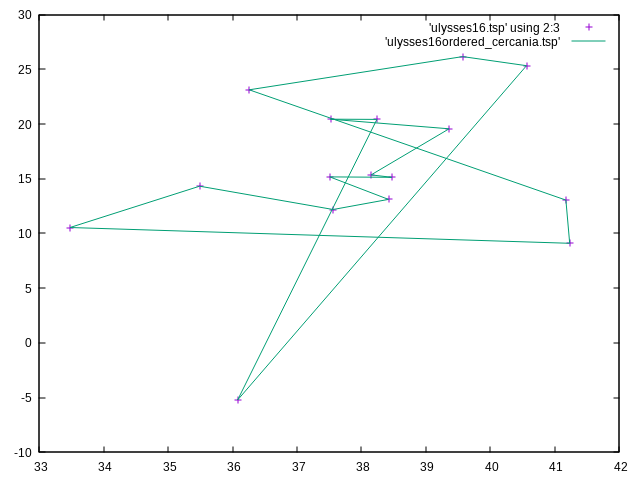
\includegraphics[scale=0.5]{./Images/ulysses_cercania.png}
	\caption{Gráfica de Ulysses mediante el Vecino más cercano}
	\end{figure}
	
	\item \texttt{bayg29.tsp}: El mejor orden para este \textit{dataset} (teniendo en cuenta el orden del fichero original) es:
	\[
		[0,27,5,11,8,4,20,1,19,9,3,14,17,13,21,16,10,18,24,6,22,26,7,23,15,12,28,25,2]
	\]
	
	y la distancia a recorrer es: 10209
	
	Si representamos los puntos con el recorrido generado obtenemos el siguiente gráfico:
	
	\begin{figure}[h!]
	\centering
	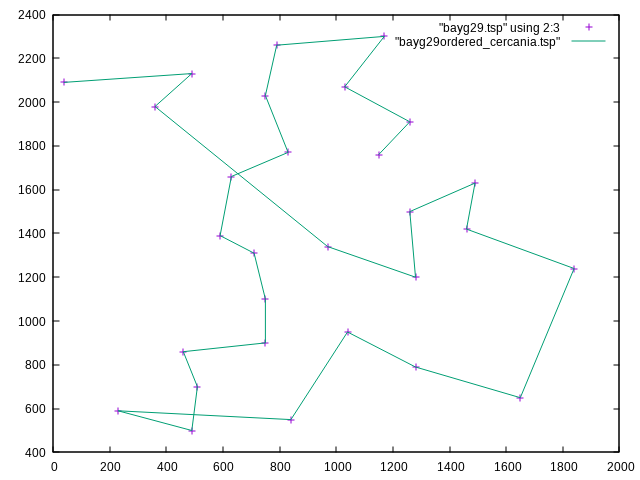
\includegraphics[scale=0.5]{./Images/bayg_cercania.png}
	\caption{Gráfica de Bayg mediante el Vecino más cercano}
	\end{figure}
	
	\newpage
	
	\item \texttt{eil76.tsp}: El mejor orden para este \textit{dataset} (teniendo en cuenta el orden del fichero original) es:
	\[
		[0,72,32,62,15,2,43,31,8,38,71,57,9,37,64,10,65,52,13,18,34,6,7,45,33,51,26,44,28,
	\]
	\[
		47,46,20,73, 27, 61,1,29,3,74,75,66,25,11,39,15,50,5,67,4,36,19,69,59,70,35,68,60,2
	\]
	\[
		1,41,40,42,22,55,48,23,17,49,24,54,30,58,53,12,56,14,63]
	\]
	
	y la distancia a recorrer es: 642
	
	Si representamos los puntos con el recorrido generado obtenemos el siguiente gráfico:
	
	\begin{figure}[h!]
	\centering
	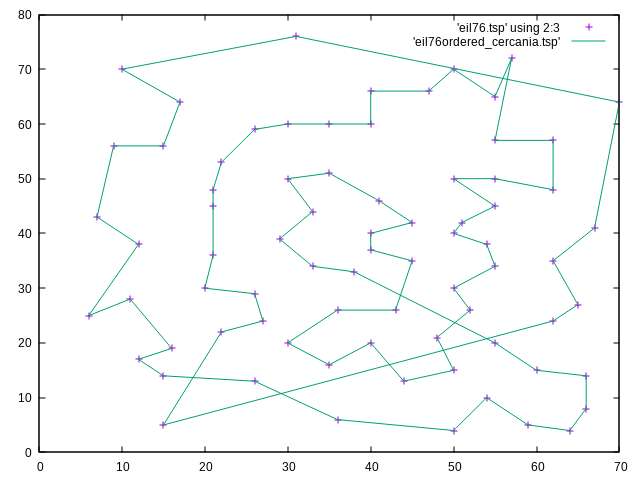
\includegraphics[scale=0.5]{./Images/eil_cercania.png}
	\caption{Gráfica de Eil mediante el Vecino más cercano}
	\end{figure}
\end{itemize}

Además, hemos obtenido más datos de problemas TSP de la página \texttt{TSPLIB} y hemos realizado un estudio con más números de ciudades y hemos medido el tiempo de ejecución de nuestro algoritmo, obteniendo los siguientes datos:


 \begin{table}[h!]
 	\centering
 	\footnotesize
 	\scalebox{0.75}{
 		\begin{tabular}{|c|c|}
 			\hline
 			\multicolumn{2}{|c|}{\textsf{Heurística del Vecino más cercano}}
 			\\\hline
 			\bfseries Ciudades (n) & \bfseries Tiempo (s)
 			\csvreader{./data/cercania_tiempo.csv}{}
 			{\\\hline\csvcoli&\csvcolii}
 			\\\hline
 		\end{tabular}
 	}
 	\caption{Experiencia empírica de el vecino más cercano}
 \end{table}

\subsubsection*{Análisis híbrido}

Después, hemos representado con \texttt{gnuplot} los datos de tiempos obtenidos en el apartado anterior y les hemos realizado un ajuste cuadrático (dato obtenido en el análisis teórico), obteniendo la gráfica que se muestra a continuación. El análisis hbirido nos permitirá comprobar que nuestro análisis teórico era correcto. 

 \begin{figure}[h!]
 	\centering
 	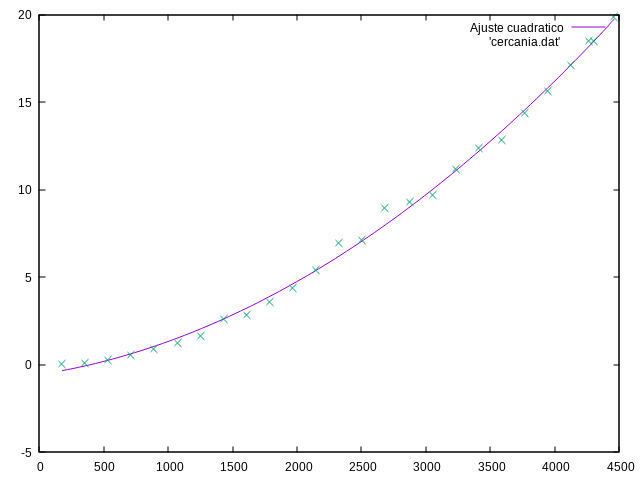
\includegraphics[scale=0.55]{./Images/cercania.png}
 	\caption{Gráfica con los tiempos de ejecución del vecino más cercano}
 \end{figure}
 
 \newpage
 
 Y las constantes ocultas son:
 \(T(n) = 7.6769 \cdot 10^{-7} n^2 + 0.00112191 n - 0.56077\)
 
 Para terminar nuesto análisis, terminaremos de confirmar que el ajuste cuadrático es el óptimo viendo el coeficiente de determinación que nos ha proporcionado gnuplot:
 
 Coef.determination = 0.869828
 
 Vemos que es un muy cercano a 1, por tanto es correcto nuestro análisis. Hay que tener en cuenta que los datos de los que partimos no son aleatorios y por tanto puede generar una pequeña perturbación en los tiempos.

\subsubsection{Heurística por inserción}
Tenemos de nuevo el mismo problema que antes del viajante del comercio pero con una heurística distinta. Veamos las 6 características de nuestro problema Greedy:
	\begin{itemize}
		\item \textbf{Un conjunto de candidatos}: En este caso, las ciudades por las que pasar.
		\item \textbf{Una lista de candidatos ya usados}: Los ciudades por las que ya se ha pasado. Cabe resaltar que se debe comenzar por un recorrido inicial de 3 ciudades previamente. Para escoger estas ciudades simplemente lo haremos escogiendo la ciudad más al oeste, la más al este y la más al norte.
		\item \textbf{Un criterio que dice cuándo un conjunto de candidatos forma una solución}: El criterio es que el recorrido que se haga forme un circuito pasando por todas las ciudades una sola vez.
		\item \textbf{Un criterio que dice cuándo un conjunto de candidatos es factible (podrá llegar a ser una solución)}: En caso de que no se repita ningún nodo (ciudad), el conjunto de candidatos es factible.
		\item \textbf{Una función de selección que indica en cualquier instante cuál es el candidato más prometedor de los no usados todavía}: Utilizaremos un criterio que denominaremos inserción mas económica: de entre todas las ciudades no visitadas, elegimos aquella que provoque el menor incremento en la longitud total del circuito.
En otras palabras, cada ciudad debemos insertarla en cada una de las soluciones posibles y quedarnos con la ciudad (y posición) que nos permita obtener un circuito de menor longitud. Seleccionaremos aquella ciudad que nos proporcione el mínimo de los mínimos calculados para cada una de las ciudades
		\item \textbf{La función objetivo que intentamos optimizar}: El coste del recorrido total del circuito.
\end{itemize}
\subsubsection*{Análisis teórico}
Visualizaremos el pseudocódigo del programa para hablar de la eficiencia:
\\
\lstinputlisting[language=C++]{./Codes/pseudocodigo_insercion.cpp}

Como se puede apreciar en el pseudocódigo, el programa recorre tres bucles distintos donde llamando n al número de ciudades, sabemos que a pesar de reduciendo el tamaño con el que se recorren los bucles, por lo visto en teoría  la función acabará teniendo eficiencia \(\mathcal{O}(n^3)\). Como aclaración la función distancia utilizada dentro del tercer bucle es  \(\mathcal{O}(1)\) y por eso no sube el orden de eficiencia.
  
  
\subsubsection*{Análisis empírico}
 Mostraremos ahora los resultados obtenidos tras probar nuestro programa con los \textit{datasets} proporcionados en la asignatura:

\begin{itemize}
	\item \texttt{ulysses16.tsp}: El mejor orden para este \textit{dataset} (teniendo en cuenta el orden del fichero original) es:
	\[
		[5, 6, 7, 10, 12, 14, 15, 13, 16, 1, 4, 8, 9, 11, 2, 3]
	\]
	
	y la distancia a recorrer es: 99
	
	Si representamos los puntos con el recorrido generado obtenemos el siguiente gráfico:
	
	\begin{figure}[h!]
	\centering
	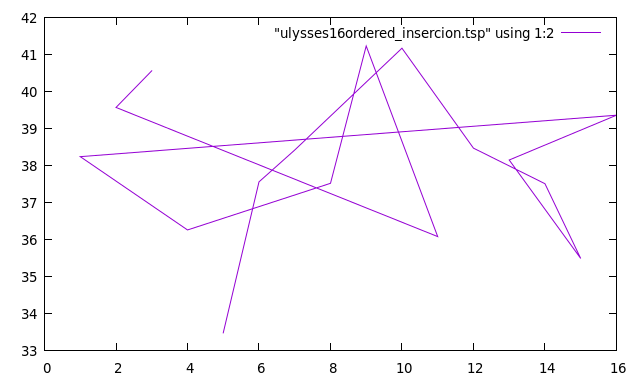
\includegraphics[scale=0.5]{./Images/ulysses_insercion.png}
	\caption{Gráfica de Ulysses mediante insercion}
	\end{figure}
	
	\newpage
	
	\item \texttt{bayg29.tsp}:  El mejor orden para este \textit{dataset} (teniendo en cuenta el orden del fichero original) es:
	\[
		[3, 23, 12, 6, 5, 26, 29, 21, 2, 20, 10, 13, 4, 15, 19, 25, 7, 18, 14, 22, 11, 17, 9, 28, 1, 24, 27, 16, 8
]
	\]
	y su distancia es 10048.

	Si representamos los puntos con el recorrido generado obtenemos el siguiente gráfico:
	\begin{figure}[h!]
	\centering
	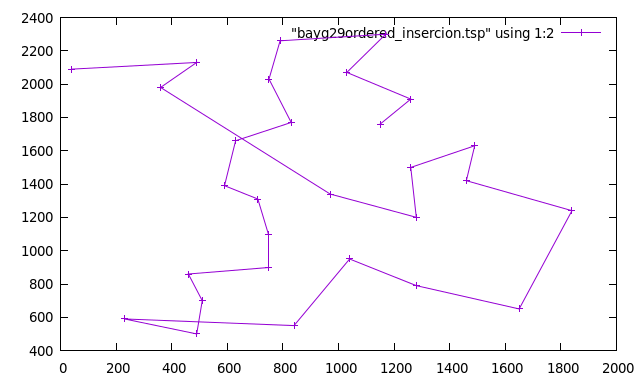
\includegraphics[scale=0.5]{./Images/bayg_insercion.png}
	\caption{Gráfica de Bayg mediante insercion}
	\end{figure}
	
	\item \texttt{eil76.tsp}:  El mejor orden para este \textit{dataset} (teniendo en cuenta el orden del fichero original) es:
	\[
		[56, 23, 63, 33, 73, 62, 22, 28, 61, 74, 30, 48, 5, 15, 57, 37, 20, 70, 60, 71, 47, 36, 69, 21, 29, 45, 27, 13, 54, 52, 34, 67, 26, 76, 75, 4, 68, 6, 51, 17, 12, 40, 46, 8, 35, 53, 11, 66, 65, 38, 10, 58, 72, 39, 9, 32, 50, 25, 55, 18, 44, 3, 14, 19, 7, 2, 1, 43, 41, 42, 64, 16, 49, 24, 59, 31
]
	\]
	y su distancia es 611.

	Si representamos los puntos con el recorrido generado obtenemos el siguiente gráfico:
	\begin{figure}[h!]
	\centering
	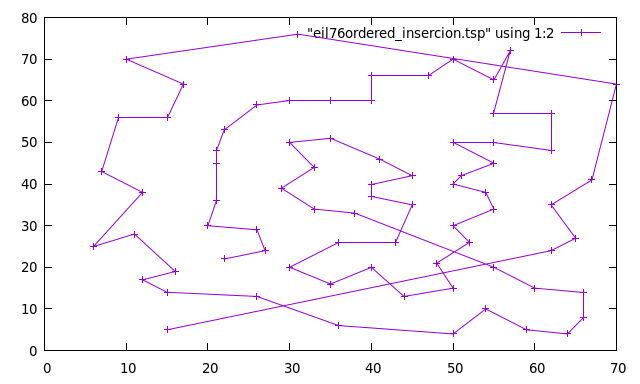
\includegraphics[scale=0.5]{./Images/eil_insercion.png}
	\caption{Gráfica de Eil mediante insercion}
	\end{figure}
  
  \end{itemize}

Además, hemos obtenido más datos de problemas TSP de la página \texttt{TSPLIB} y hemos realizado un estudio con más números de ciudades y hemos medido el tiempo de ejecución de nuestro algoritmo, obteniendo los siguientes datos:


 \begin{table}[h!]
 	\centering
 	\footnotesize
 	\scalebox{0.75}{
 		\begin{tabular}{|c|c|}
 			\hline
 			\multicolumn{2}{|c|}{\textsf{Heurística de inserción}}
 			\\\hline
 			\bfseries Ciudades (n) & \bfseries Tiempo (s)
 			\csvreader{./data/insercion_tiempo.csv}{}
 			{\\\hline\csvcoli&\csvcolii}
 			\\\hline
 		\end{tabular}
 	}
 	\caption{Experiencia empírica de inserción}
 \end{table}

\subsubsection*{Análisis híbrido}

Después, hemos representado con \texttt{gnuplot} los datos de tiempos obtenidos en el apartado anterior y les hemos realizado un ajuste cuadrático (dato obtenido en el análisis teórico), obteniendo la gráfica que se muestra a continuación. El análisis hbirido nos permitirá comprobar que nuestro análisis teórico era correcto. 

 \begin{figure}[h!]
 	\centering
 	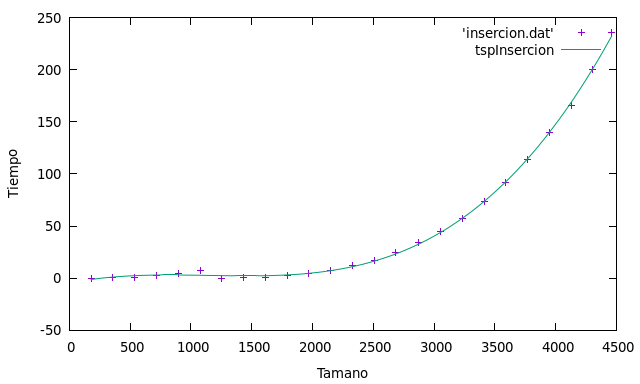
\includegraphics[scale=0.55]{./Images/insercion.png}
 	\caption{Gráfica con los tiempos de ejecución de insercion}
 \end{figure}
 
 \newpage
 
 Y las constantes ocultas son:
 \(T(n) = 6.46703 \cdot 10^{-9} n^3 - 2.21761 \cdot 10^{-5} n^2 + 0.02336 n - 4.75186 \)
 
 Para terminar nuesto análisis, terminaremos de confirmar que el ajuste cúbico es el óptimo viendo el coeficiente de determinación que nos ha proporcionado gnuplot:
 
 Coef.determination = 0.85647
 
 Vemos que es un muy cercano a 1, por tanto es correcto nuestro análisis. Hay que tener en cuenta que los datos de los que partimos no son aleatorios y por tanto puede generar una pequeña perturbación en los tiempos.

\subsubsection{Heurística propia: perturbaciones}

Este enfoque, de nuevo \textit{greedy}, realiza las perturbaciones indicadas por un parámetro sobre un recorrido dado para intentar mejorarlo. Tenemos el siguiente código:
\lstinputlisting[language=Python]{./Codes/perturbaciones.py}

\subsubsection*{Análisis teórico}

Primero lo que hacemos es obtener una solución mediante la heurística del vecino más cercano. Tras esto, tenemos la función \texttt{get\_worst\_node} que es \(\mathcal{O}(n)\), que dado un recorrido, haya el nodo que más dista de su nodo siguiente. Por ello es necesario usar ya una solución previa (mediante el vecino más cercano) para calcular este ``nodo peor''. Por último, tenemos la función \texttt{perturbate} que es \(\mathcal{O}(n^2)\), que prueba todas las posibles permutaciones que podemos hacer desde el respectivo ``peor nodo'' y se queda con la mejor de ellas. Por todo ello, apoyándonos en los comentarios realizados en el código mostrado, podemos concluir que:
\[
	T(n) \in \mathcal{O}(n^2 \cdot perturbaciones) \Rightarrow T(n) \in \mathcal{O}(n^2)
\]

\subsubsection*{Análisis empírico}

A continuación, mostramos los resultados obtenidos tras probar nuestro programa con los \textit{datasets} proporcionados en la asignatura:
\begin{itemize}
	\item \texttt{ulysses16.tsp}: Aplicando 10 perturbaciones, obtenemos que el mejor orden (teniendo en cuenta el orden del fichero original):
	\[
		[0,7,15,12,11,13,6,5,14,4,8,9,2,1,3,10]
	\]
	y su distancia es 101.

	Si representamos los puntos con el recorrido generado para 10 perturbaciones obtenemos el siguiente gráfico:
	\begin{figure}[h!]
	\centering
	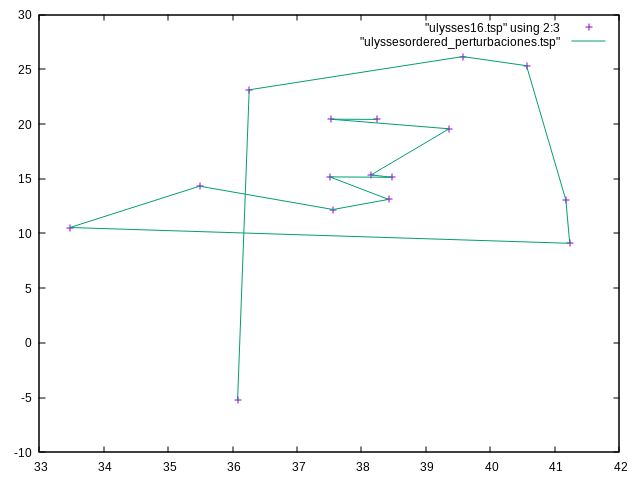
\includegraphics[scale=0.5]{./Images/ulysses_perturbaciones.png}
	\caption{Gráfica de Ulysses mediante perturbaciones}
	\end{figure}
	
	\newpage
	
	\item \texttt{bayg29.tsp}: Aplicando 10 perturbaciones, obtenemos que el mejor orden (teniendo en cuenta el orden del fichero original):
	\[
		[0,27,5,11,8,4,20,1,19,9,3,14,17,13,21,16,10,18,24,6,22,26,7,23,15,12,28,25,2]
	\]
	y su distancia es 10209.

	Si representamos los puntos con el recorrido generado para 10 perturbaciones obtenemos el siguiente gráfico:
	\begin{figure}[h!]
	\centering
	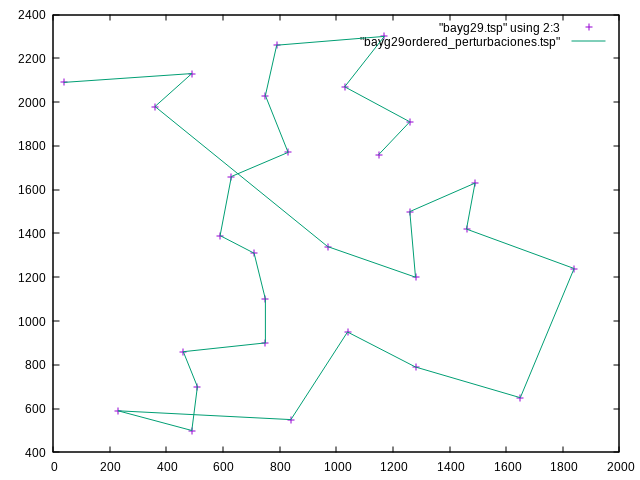
\includegraphics[scale=0.5]{./Images/bayg_perturbaciones.png}
	\caption{Gráfica de Bayg mediante perturbaciones}
	\end{figure}
	
	\item \texttt{eil76.tsp}: Aplicando 10 perturbaciones, obtenemos que el mejor orden (teniendo en cuenta el orden del fichero original):
	\[
		[0,72,32,62,15,2,43,31,8,38,71,57,9,37,64,10,65,52,13,18,34,6,7,45,33,51,26,44,28,
	\]
	\[
		47,46,20,73,27,61,1,29,3,74,75,66,25,11,39,16,50,5,67,4,36,19,69,59,70,35,68,60,2,
	\]
	\[
		1,41,40,42,22,55,48,23,17,49,24,54,30,58,53,12,56,14,63]
	\]
	y su distancia es 642.

	Si representamos los puntos con el recorrido generado para 10 perturbaciones obtenemos el siguiente gráfico:
	
	\newpage
	\begin{figure}[h!]
	\centering
	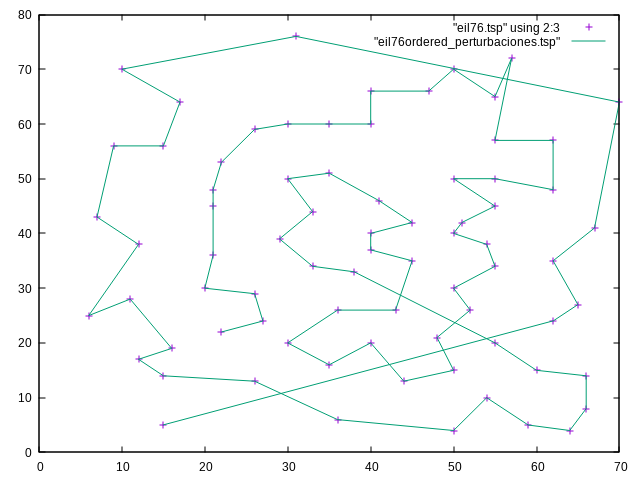
\includegraphics[scale=0.5]{./Images/eil_perturbaciones.png}
	\caption{Gráfica de Eil mediante perturbaciones}
	\end{figure}
\end{itemize}

Además. hemos obtenido más de problemas TSP de la página \texttt{TSPLIB} y hemos realizado un estudio con más números de ciudades y hemos medido el tiempo de ejecución de nuestro algoritmo, obteniendo los siguientes datos:

 \begin{table}[h!]
 	\centering
 	\footnotesize
 	\scalebox{0.75}{
 		\begin{tabular}{|c|c|}
 			\hline
 			\multicolumn{2}{|c|}{\textsf{Heurística de perturabciones}}
 			\\\hline
 			\bfseries Ciudades (n) & \bfseries Tiempo (s)
 			\csvreader{./data/perturbaciones_tiempo.csv}{}
 			{\\\hline\csvcoli&\csvcolii}
 			\\\hline
 		\end{tabular}
 	}
 	\caption{Experiencia empírica de perturbaciones}
 \end{table}
 
 \subsubsection*{Análisis híbrido}
 
Después, hemos representado con \texttt{gnuplot} los datos de tiempo obtenidos en el apartado anterior y les hemos realizado un ajuste cuadrático (dato obtenido en el análisis teórico), obteniendo la gráfica que se muestra a continuación. El análisis híbrido nos permitirá comprobar que nuestro análisis teórico era correcto.

\begin{figure}[h!]
 	\centering
 	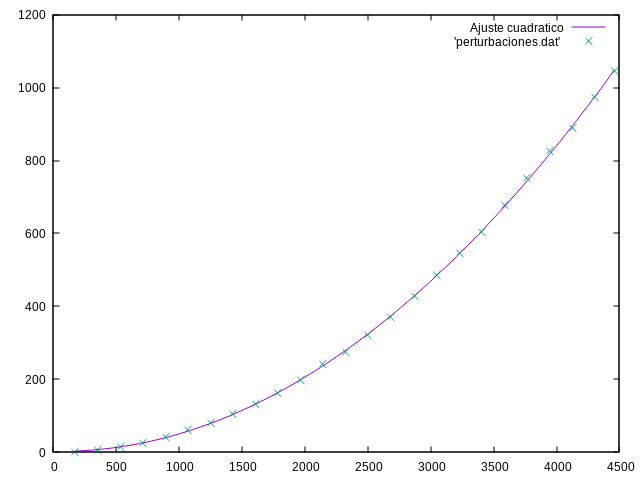
\includegraphics[scale=0.55]{./Images/perturbaciones.png}
 	\caption{Gráfica con los tiempos de ejecución de perturbaciones}
 \end{figure}
 
 \newpage
 
 Y las constantes ocultas son \(T(n) = 5.39602 \cdot 10^{-5} \cdot n^2 - 0.00659642 n + 3.2468\).
 
 Para terminar nuestro análisis, terminaremos de confirmar que el ajuste cuadrático es el óptimo viendo el coeficiente de determinación que nos ha proporcionado gnuplot:
 
 Coef.determination = 0.93507
 
 Vemos que es muy cercano a 1, por tanto nuestro análisis es correcto.

\subsubsection{Comparación de heurísticas}

Los tres algoritmos que tenemos son: cercanía (el vecino más cercano), inserción y por perturbaciones. Veremos la gráfica comparativa de los tiempos de cada heurística.

\begin{figure}[h!]
 	\centering
 	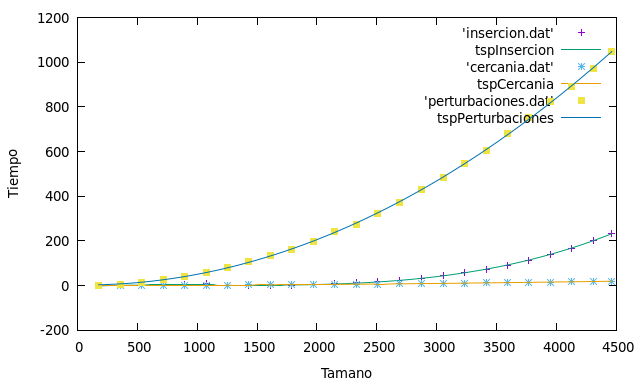
\includegraphics[scale=0.55]{./Images/comparativa_tiempos.png}
 	\caption{Gráfica comparativa con los tiempos de ejecución de las distintas heurísticas}
 \end{figure}
 
 Vemos como los tiempos de ejecución son mayores para inserción debido a que su eficiencia es cúbica respecto a los demás, donde también se observa que la heurística de perturbaciones tiene un tiempo algo mayor que la de cercanía. Sin embargo este mayor tiempo se puede justificar a la hora de escoger estas heurísticas debido a que el algoritmo que proporciona mejores soluciones es, como se puede comprobar con los costes previamente reflejados, el que utiliza la heurística de inserción y posteriormente al que utiliza la heurística de perturbaciones. Por tanto la conclusión en este caso es que a mayor tiempo de ejecución mejor solución obtenemos y por tanto debemos de tener esto en cuenta a la hora de elegir una heurística u otra.

\section{Conclusiones}

Con esta práctica, hemos aprendido a crear algoritmos voraces para resolver problemas que, en su versión obvia o de fuerza bruta tienen una complejidad en ocasiones demasiado elevadas.

Además, hemos comprobado como dentro de esta misma técnica podemos atacar los problemas de manera distinta. Debemos de prestar atención a la dificultad de obtener la solución óptima, y primar el ``acercarnos'' a ella mediante algoritmos que van mejorando la solución anterior.

Esto es algo de especial relevancia a la hora de trabajar con cantidades ingentes de datos, en el que dar una solución inicial puede ser muy complicado, pudiendo partir incluso de soluciones arbitrarias, mejorándolas conforme nuestros algoritmos se van ejecutando. 
\end{document}